\begin{frame}
 \frametitle{Diffusion across synapses}
 \begin{columns}
\column{0.48\textwidth}
 \begin{itemize}
 \item Two types of synapses connect neurons - electrical and chemical.
 \item Action potentials triggers release of neurotransmitter into synaptic cleft.
 \item Receiving end passes input on to cell body.
 \item Diffusion across synaptic cleft takes $\sim\mu$s or less.
 \end{itemize}
\column{0.48\textwidth}
\begin{figure}[H]
 \centering
 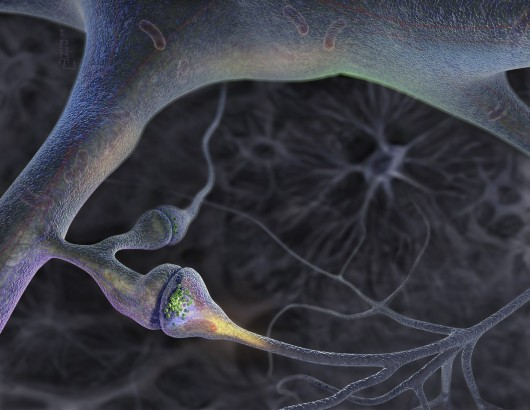
\includegraphics[width=\textwidth]{figures/synapse.jpg}
 \caption{Chemical synapse with dendritic spine.}
\end{figure}
 \end{columns} 
\end{frame}

\begin{frame}
 \frametitle{PKC$\gamma$ diffusion into spines}
 \begin{columns}
  \column{2.0in}
  \begin{itemize}
   \item PKC$\gamma$ is an enzyme associated with learning.
   \item Released from cell body and diffuses through dendrite into spines.
   \item Very low concentrations could require multi scale modeling.
  \end{itemize}
\column{2.0in}
\begin{figure}[H]
\centering
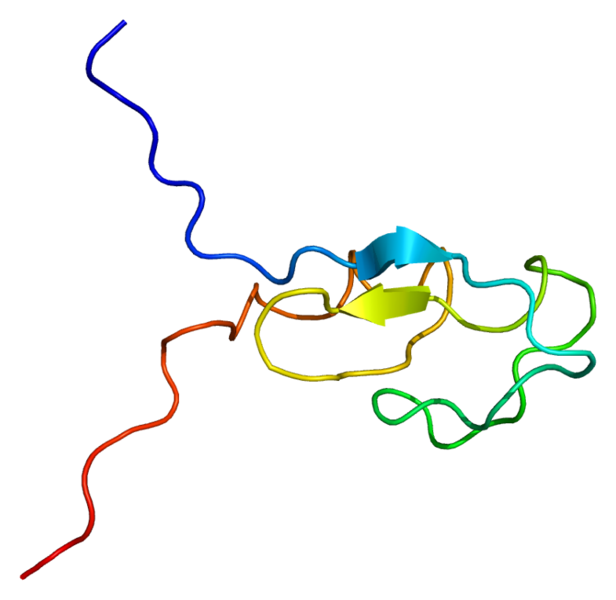
\includegraphics[width=\textwidth]{figures/PKCG.png}
\end{figure}

 \end{columns}

\end{frame}
